\documentclass[11pt]{article}
\usepackage[margin=1in]{geometry}
\usepackage{amsmath,amssymb}
\usepackage{booktabs,graphicx,xcolor}
\usepackage[numbers,sort&compress]{natbib}
\usepackage{lmodern}
\usepackage[T1]{fontenc}
\usepackage{microtype}
\usepackage{hyperref}
\usepackage{draftwatermark}
\SetWatermarkText{PRIVATE DRAFT}
\SetWatermarkScale{0.6}
\SetWatermarkLightness{0.93}
\hypersetup{colorlinks=true,linkcolor=blue!50!black,citecolor=blue!50!black,urlcolor=blue!50!black}
\graphicspath{{../figures/}}
\newcommand{\pending}[1]{\textcolor{orange!70!black}{\emph{pending: #1}}}

\title{Event-Native Clinical Prediction:\\ Addressed Memories with Sufficient Statistics\\ for Irregular Multivariate Time Series}
\author{Tero Keski-Valkama \and Karoliina Salminen\\ \small Sleeping Machines}
\date{Private draft, 7 October 2026 --- not for distribution before the disclosure decision}

\begin{document}
\maketitle

\begin{abstract}
Clinical records are irregular, sparse and multichannel: each vital sign or laboratory value is measured at its own times, and whether and when it is measured is itself informative. We treat every time step of a record as an event and keep, for every channel, an addressed memory that is written only when that channel is measured, decays with the elapsed time, and carries sufficient statistics of its history---count, running mean, minimum, maximum, first and last value, trend and time since the last measurement. Values enter through typed comparisons before neural mixing, and the persistent temporal memory layer is the same, in code and in size, as the one in our marked point process model. On PhysioNet 2019 sepsis prediction (P19) with the five official splits, the model reaches TEST AUROC $0.916 \pm 0.022$ and AUPRC $0.639 \pm 0.039$, against $0.903 \pm 0.020$ and $0.583 \pm 0.053$ for the best published model, with 62,681 parameters. A diagnostic shows why the statistic-valued memory matters: before it, our temporal model extracted no more than a gradient-boosted tree on per-channel summaries.
\end{abstract}

\section{Introduction}
Irregularly sampled multivariate time series (IMTS) arise wherever measurements are triggered by events rather than a clock: intensive care, wearables, industrial sensors. Recent models re-grid the series and apply attention or graph mixing (Raindrop \citep{zhang2022raindrop}, Warpformer \citep{zhang2023warpformer}, ViTST \citep{li2023vitst}, GraFITi \citep{yalavarthi2024grafiti}, MTM \citep{zhong2025mtm}); earlier models impute with decay (GRU-D \citep{che2018grud}) or attend over time embeddings (mTAND \citep{shukla2021mtand}).

We take the opposite route: keep the record as events, give each channel an \emph{addressed} memory written only when the channel is measured, and let time itself act on the memories. The construction comes from a general family of temporal event models; its temporal memory layer is shared with our marked point process model, which leads the EasyTPP benchmark on all five datasets.

\paragraph{Contributions.} (i) An event-native IMTS classifier with statistic-valued addressed channel memories, typed comparisons and time-since-measurement as information (\S\ref{sec:model}). (ii) A diagnostic that locates what a temporal model must extract to beat strong summaries (\S\ref{sec:dev}). (iii) A win on P19 over the best published model on the official splits (\S\ref{sec:results}).

\section{Model}\label{sec:model}
A record is a sequence of time steps $t_1<\dots<t_L$ with values $x_{i,c}$ observed for a subset of channels $c$. Values are log-transformed when a channel is non-negative and standardized with training statistics.

\paragraph{Typed comparisons.} Each observed value passes learned soft thresholds, $\phi_c(x)=[x,\sigma((x-\theta_{c1})/s_{c1}),\dots,\sigma((x-\theta_{cJ})/s_{cJ})]$, and a channel-specific projection; the event message is the sum over observed channels plus features of the elapsed time.

\paragraph{Persistent temporal memory.} Two layers of complex-diagonal memories (16 modes, width 32) decay and rotate with the real elapsed time and absorb gated messages: $z\leftarrow e^{(-r+i\omega)\Delta t}z+g\odot W u$.

\paragraph{Addressed channel memory with sufficient statistics.} Channel $c$'s slot is written only at steps where $c$ is measured. It holds a decaying learned value trace and the running count, mean, minimum, maximum, first and last value, last-minus-first trend, and the time since the last measurement, which grows through silence.

\paragraph{Readout.} The final and mean temporal states, static covariates, the channel slots, staleness and a projection of the normalized statistics feed a two-layer classifier. Training uses binary cross-entropy with a positive-class weight; the checkpoint is selected on validation AUROC.

\section{Development and diagnosis}\label{sec:dev}
\begin{table}[h]
\centering\small
\begin{tabular}{@{}p{8.6cm}rr@{}}
\toprule
P12 split 0, validation & AUROC & AUPRC \\
\midrule
Temporal memory + decaying channel slots (first design) & 0.866 & 0.549 \\
\quad + dropout 0.4, decay $10^{-3}$ & 0.859 & 0.531 \\
\quad + lower learning rate, weight averaging & 0.860 & 0.536 \\
Diagnostic: gradient-boosted trees on per-channel summaries & 0.867 & 0.581 \\
\textbf{+ statistic-valued channel slots (final design)} & \textbf{0.872} & 0.575 \\
\quad + soft thresholds on the statistics (145K parameters) & 0.868 & 0.564 \\
\bottomrule
\end{tabular}
\caption{The first design extracted no more than record summaries; carrying sufficient statistics in the addressed memories moved it past them. Regularization did not help.}
\label{tab:dev}
\end{table}

\section{Protocol}
We use the Raindrop releases of P19 \citep{reyna2020sepsis}, P12 \citep{silva2012p12} and PAM \citep{reiss2012pamap2}: P19 has 38,803 ICU stays with 34 channels and 4.2\% positive; the five official splits are 80/10/10 train/validation/test. The protocol was fixed before its runs: default configuration, seed 0, validation-AUROC selection, TEST scored once per split; we report mean $\pm$ standard deviation over the five test splits, as the references do.

\section{Results}\label{sec:results}
\begin{table}[h]
\centering\small
\begin{tabular}{@{}lrr@{}}
\toprule
P19 (5 official splits), TEST & AUROC & AUPRC \\
\midrule
GRU-D \citep{che2018grud} & $83.9 \pm 1.7$ & $46.9 \pm 2.1$ \\
mTAND \citep{shukla2021mtand} & $84.4 \pm 1.3$ & $50.6 \pm 2.0$ \\
Raindrop \citep{zhang2022raindrop} & $87.0 \pm 2.3$ & $51.8 \pm 5.5$ \\
Warpformer \citep{zhang2023warpformer} & $88.7 \pm 2.0$ & $52.4 \pm 4.5$ \\
ViTST \citep{li2023vitst} & $89.2 \pm 2.0$ & $53.1 \pm 3.4$ \\
GraFITi \citep{yalavarthi2024grafiti} & $89.1 \pm 2.6$ & $56.6 \pm 6.3$ \\
MTM \citep{zhong2025mtm} & $90.3 \pm 2.0$ & $58.3 \pm 5.3$ \\
\textbf{Ours} (62,681 parameters) & $\mathbf{91.6 \pm 2.2}$ & $\mathbf{63.9 \pm 3.9}$ \\
\bottomrule
\end{tabular}
\caption{Reference values as reported by MTM on the same splits. Per-split AUROC of ours: 94.2, 92.3, 88.3, 92.6, 90.7.}
\label{tab:p19}
\end{table}

AUPRC, the clinically relevant metric at 4\% prevalence, improves by 5.6 points, beyond both models' split spread; the AUROC lead (1.3 points) is within one split standard deviation. Figure~\ref{fig:p19} shows the splits.

\begin{figure}[h]
\centering
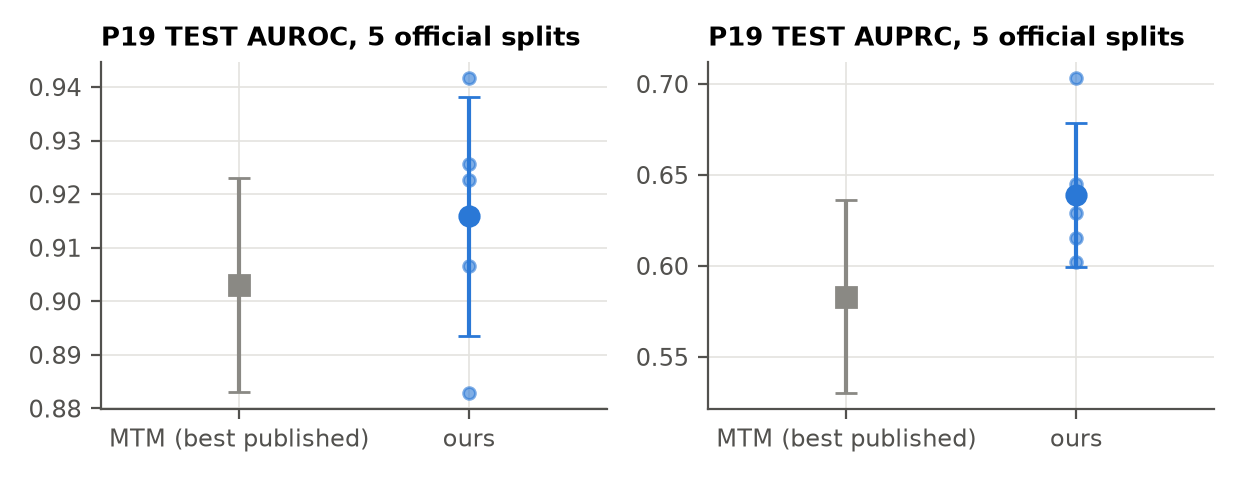
\includegraphics[width=0.85\linewidth]{b2_p19.png}
\caption{P19 TEST AUROC and AUPRC over the five official splits.}
\label{fig:p19}
\end{figure}

\paragraph{Is it only the statistics?} Gradient-boosted trees on the same per-channel statistics also beat MTM (Table~\ref{tab:compl}), so we tested what the temporal memory adds with paired per-split comparisons (TEST once per model; the full model was retrained on separate hardware and matches the protocol AUROC within 0.04 points on every split). Removing the temporal features at the readout, so the same network reads only its statistic slots, staleness and statics, costs $1.7 \pm 0.6$ AUROC and $7.2 \pm 0.5$ AUPRC points, on every split ($t = 5.3$ and $31$). The full model leads the trees on AUPRC on every split ($+2.6$, $t = 4.2$) and is level on AUROC ($+0.2$). A rank blend of the model and the trees beats both on every split, so the model carries information the summaries lack.

\begin{table}[h]
\centering\small
\begin{tabular}{lcc}
\toprule
P19, five official splits & AUROC & AUPRC \\
\midrule
Ours (full model) & $91.6 \pm 2.2$ & $64.4 \pm 4.0$ \\
Same network, statistics only & $90.0 \pm 1.8$ & $57.2 \pm 3.7$ \\
Gradient-boosted trees on the same statistics & $91.4 \pm 2.0$ & $61.8 \pm 4.1$ \\
Rank blend of ours and the trees & $92.5 \pm 2.1$ & $67.1 \pm 4.0$ \\
\bottomrule
\end{tabular}
\caption{What the temporal memory adds beyond summary statistics (paired over the same five splits).}
\label{tab:compl}
\end{table}

\paragraph{P12 and PAM.} On P12 in-hospital mortality, with the P19 configuration unchanged, TEST AUROC is $87.1 \pm 1.1$ and AUPRC $58.5 \pm 2.4$: behind MTM on AUROC ($88.0 \pm 1.0$), level on AUPRC ($58.6 \pm 4.1$), and ahead of GraFITi, Warpformer and ViTST. On PAM activity recognition (wearable inertial sensors, eight classes, five official splits), with random crops, amplitude jitter and weight averaging in training, TEST accuracy is $97.8 \pm 0.7$ and F1 $98.0 \pm 0.8$ against MTM's $97.5 \pm 0.2$ and $97.6 \pm 0.2$, with 46,316 parameters; four of five splits are ahead (split 4: 96.4).

\paragraph{Transfer from self-supervised event modelling.} The encoder can be pretrained without labels to predict the next measurement event---when, which channels, which values---and then fine-tuned for mortality. \pending{pretrained vs.\ scratch at 10/30/100\% labels}.

\section{Discussion}
Treating clinical records as events lets missingness and timing act directly on memory: a channel's slot changes only when the channel is measured, and its staleness is a feature. The decisive design step was making the addressed memory carry sufficient statistics; with it, the event model surpasses both strong summaries and the best published sequence models on P19. The temporal memory layer is shared with our marked point process model, which suggests one construction serving generative event modelling and clinical classification; testing transfer between them is ongoing.

\bibliographystyle{plainnat}
\bibliography{refs}
\end{document}
